\documentclass[11pt]{article}
\usepackage[utf8]{inputenc}
\usepackage{textcomp}
\usepackage{listings}
\usepackage{tikz}
\usepackage{enumerate}
\usepackage{url}
%\usepackage{algorithm2e}
\usetikzlibrary{arrows,automata,shapes}
\tikzstyle{block} = [rectangle, draw, fill=blue!20, 
    text width=5em, text centered, rounded corners, minimum height=2em]
\tikzstyle{bt} = [rectangle, draw, fill=blue!20, 
    text width=1em, text centered, rounded corners, minimum height=2em]

\lstset{ %
  basicstyle=\ttfamily,commentstyle=\scriptsize\itshape,showstringspaces=false,breaklines=true,numbers=none}
\lstset{
     literate=%
         {á}{{\'a}}1
         {í}{{\'i}}1
         {é}{{\'e}}1
         {ý}{{\'y}}1
         {ú}{{\'u}}1
         {ó}{{\'o}}1
         {ě}{{\v{e}}}1
         {š}{{\v{s}}}1
         {č}{{\v{c}}}1
         {ř}{{\v{r}}}1
         {ž}{{\v{z}}}1
         {ď}{{\v{d}}}1
         {ť}{{\v{t}}}1
         {ň}{{\v{n}}}1                
         {ů}{{\r{u}}}1
         {Á}{{\'A}}1
         {Í}{{\'I}}1
         {É}{{\'E}}1
         {Ý}{{\'Y}}1
         {Ú}{{\'U}}1
         {Ó}{{\'O}}1
         {Ě}{{\v{E}}}1
         {Š}{{\v{S}}}1
         {Č}{{\v{C}}}1
         {Ř}{{\v{R}}}1
         {Ž}{{\v{Z}}}1
         {Ď}{{\v{D}}}1
         {Ť}{{\v{T}}}1
         {Ň}{{\v{N}}}1                
         {Ů}{{\r{U}}}1    
}

\newtheorem{defn}{Definition}
\newtheorem{crit}{Criterion}

\newcommand{\handout}[5]{
  \noindent
  \begin{center}
  \framebox{
    \vbox{
      \hbox to 5.78in { {\bf Intro to Methods of Software Engineering } \hfill #2 }
      \vspace{4mm}
      \hbox to 5.78in { {\Large \hfill #5  \hfill} }
      \vspace{2mm}
      \hbox to 5.78in { {\em #3 \hfill #4} }
    }
  }
  \end{center}
  \vspace*{4mm}
}

\newcommand{\lecture}[4]{\handout{#1}{#2}{#3}{#4}{Lecture #1}}
\topmargin 0pt
\advance \topmargin by -\headheight
\advance \topmargin by -\headsep
\textheight 8.9in
\oddsidemargin 0pt
\evensidemargin \oddsidemargin
\marginparwidth 0.5in
\textwidth 6.5in

\parindent 0in
\parskip 1.5ex
%\renewcommand{\baselinestretch}{1.25}

\newcommand{\squishlist}{
 \begin{list}{$\bullet$}
  { \setlength{\itemsep}{0pt}
     \setlength{\parsep}{3pt}
     \setlength{\topsep}{3pt}
     \setlength{\partopsep}{0pt}
     \setlength{\leftmargin}{1.5em}
     \setlength{\labelwidth}{1em}
     \setlength{\labelsep}{0.5em} } }
\newcommand{\squishlisttwo}{
 \begin{list}{$\bullet$}
  { \setlength{\itemsep}{0pt}
     \setlength{\parsep}{0pt}
    \setlength{\topsep}{0pt}
    \setlength{\partopsep}{0pt}
    \setlength{\leftmargin}{2em}
    \setlength{\labelwidth}{1.5em}
    \setlength{\labelsep}{0.5em} } }
\newcommand{\squishend}{
  \end{list}  }

\begin{document}

\lecture{10 --- November 15, 2016}{Fall 2016}{Patrick Lam}{version 1}

\begin{center}
``With great power there must also come great responsibility\footnote{\url{http://quoteinvestigator.com/2015/07/23/great-power/}.}''

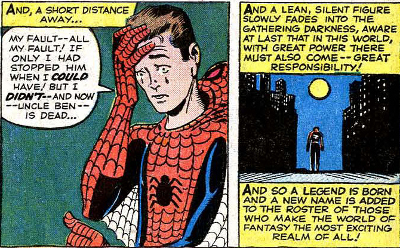
\includegraphics{images/spider400.jpg}
\end{center}

Today's topic is professional responsibility. Of course, engineers
have a responsibility to not design bridges that fall down, but none
of you are going to design bridges. However, some of you are likely to
work at Facebook, and we'll talk about them today. My objective is to
provoke thought.

%% ; specifically, in the first
%% segment of the class, you will explore the following questions:

%% \begin{itemize}
%% \item what are Facebook's goals?
%% \item how can Facebook affect society?
%% \item how does that affect its actions?
%% \end{itemize}

Engineers have a responsibility to the public. The question that comes up, then, is
what should Facebook do with its responsibility.

I want to start by examining Facebook's motives. We've shot a glancing
look at Facebook's motives earlier in the term, but I want to examine
this in more depth.

\begin{itemize}
\item As a corporation, what is Facebook primarily trying to do?
\item How does it make money?
\item How does it make more money?
\end{itemize}

\paragraph{Group discussion 1.} How can Facebook affect behaviour, and
how do we know that Facebook affects behaviour? This part of the
assignment is a research assignment; find some evidence to support
this claim, cite it, and summarize it in one paragraph. (15 minutes)

\paragraph{Group discussion 2.} Let's discuss the implications of changes in FB's news feed
algorithm.  The exercise is to propose any change (e.g. only show
posts with green pictures, show posts randomly) to FB's news ranking
algorithm, and discuss the economic, social and technological
implications. (15 minutes)

\paragraph{Group discussion 3.} The final part of today's discussion will explore Facebook's
responsibilities with respect to the public interest. Let's first
talk about responsibility to the public in general. Clearly, 
you mustn't design bridges that are going to cause harm to the public.
Facebook isn't going to literally fall on anyone's head, but it can
still cause harm to the public.

We could talk about abstract harms, but let's keep it concrete. I'd like
you to look up specific examples. Categories of harms include cyberbullying,
misinformation, and locking people out of their accounts. (15 minutes)

\paragraph{Summary.}
We started class today by talking about social responsibility versus Facebook
profits. In some ways, these work at cross purposes: one can maximize profits while 
abdicating social responsibility. But I don't believe that the world actually works
that way. A prosperous, healthy society is going to produce more long-term profits
than a dysfunctional society. 

As an individual contributor, social responsibility is not generally something
that you will think about every day. But it is important, and there will be times
in your career when you can make a difference. Please, look out for those times,
and do the right thing when you can.

\paragraph{Digression.} By the way\ldots

\scriptsize
\begin{center}
\url{http://www.laweekly.com/restaurants/why-yelp-s-chinese-restaurant-ratings-don-t-compute-7603048}
\end{center}


\end{document}
